\documentclass[11pt]{article}

% ============================================================
%  Pr_t Calibration Diagnostics -- Technical Memo
%  Mach 14 flat-plate, cold-wall RANS calibration
%  Self-contained summary for future reference.
% ============================================================

\usepackage[a4paper,margin=1in]{geometry}
\usepackage{amsmath,amssymb}
\usepackage{graphicx}
\usepackage{booktabs}
\usepackage{float}
\usepackage{xcolor}
\usepackage{siunitx}
\usepackage[colorlinks=true,linkcolor=blue!60!black,urlcolor=blue!60!black]{hyperref}
\usepackage{enumitem}
\usepackage{caption}
\captionsetup{font=small,labelfont=bf}

\graphicspath{{./}}

\definecolor{accent}{RGB}{20,80,140}
\newcommand{\Prt}{\ensuremath{Pr_t}}
\newcommand{\utau}{\ensuremath{u_\tau}}

\title{\textbf{Calibration Diagnostics for the Turbulent Prandtl Number}\\[2pt]
\large Mach 14 Cold-Wall Flat-Plate Boundary Layer (RANS / Spalart--Allmaras)}
\author{Matar Hedi \\ \small Advisor: Prof.\ Steven Frankel}
\date{\today}

\begin{document}
\maketitle

\begin{abstract}
\noindent
This memo documents an investigation triggered by a single strategic question:
\emph{is the turbulent Prandtl number (\Prt) calibration a real, physically meaningful
engineering result, or could it be a fudge factor compensating for other model
errors?} A velocity-profile mismatch between RANS and DNS raised the concern that the
heat-flux error might originate in the momentum field rather than in \Prt.
We built three independent diagnostics and a wall-shear forensic study. The verdict:
the \Prt{} calibration is physically sound \emph{in the space where it is performed}
(the self-similar temperature--velocity relation), recovering a value
($\Prt = 0.566$) close to the DNS-measured boundary-layer average ($0.639$). With a
corrected, DNS-consistent baseline (freestream Reynolds number \emph{derived} from the
DNS state rather than an ad-hoc fixed value), the velocity-space discrepancy that
triggered the concern is largely resolved: in wall units the RANS momentum field now
collapses onto the DNS/log-law (friction velocity $\utau = \SI{63.2}{m/s}$ vs DNS
$\SI{67.6}{m/s}$). The residual difference is a benign Reynolds-number/flow-state gap
(the RANS boundary layer is still developing), not a turbulence-model failure. The
remaining actionable issue is deeper energy-equation convergence in the stored baseline
run.
\end{abstract}

% ============================================================
\section{Motivation: Is This a Real and Novel Problem?}
% ============================================================
The thesis automates the calibration of \Prt{} in RANS turbulence models for hypersonic
cold-wall boundary layers. Before investing further, we stress-tested the premise.

\paragraph{Why \Prt{} is the correct knob.}
In RANS the turbulent heat flux is closed by a gradient-diffusion hypothesis,
\begin{equation}
q_t = -\rho\, c_p\, \frac{\nu_t}{\Prt}\,\frac{\partial T}{\partial y},
\end{equation}
where the eddy viscosity $\nu_t$ comes from the \emph{momentum} model (Spalart--Allmaras).
\Prt{} is therefore the single closure coefficient that converts the (already computed)
momentum turbulence into heat transport---the Reynolds analogy, hard-coded as
$\Prt \approx 0.9$. It is the minimal, physically targeted correction to the thermal
field that does not disturb the (good) velocity prediction.

\paragraph{What is and is not novel.}
That \Prt{} departs from $0.9$ in hypersonic cold-wall flow is \emph{known} physics.
The novelty of the thesis is the \emph{methodology}: an automated, data-driven,
sample-efficient (Gaussian-Process + Active-Learning) inverse-calibration pipeline that
maps flow conditions to optimal \Prt{}, validated against a DNS family, and its
generalization to new geometries (compression ramp / SBLI). The underlying engineering
problem---accurate hypersonic aeroheating for thermal-protection-system design---is real
and high value.

\paragraph{The headline result (Mach 14).}
\begin{table}[H]
\centering
\begin{tabular}{lccc}
\toprule
Metric & Standard ($\Prt=0.9$) & Calibrated ($\Prt=0.566$) & Change \\
\midrule
$T/U$ RMSE vs DNS      & 0.739 & 0.286 & $\mathbf{-61.3\%}$ \\
Wall heat flux         & \SI{0.94}{kW/m^2} & \SI{0.73}{kW/m^2} & $-22\%$ \\
Velocity RMSE vs DNS   & $\sim 0.22$ & $\sim 0.22$ & unchanged \\
\bottomrule
\end{tabular}
\caption{Validated single-condition calibration result. Source: \texttt{optimization\_log.csv}.}
\end{table}

% ============================================================
\section{The Concern and the Key Insight}
% ============================================================
\paragraph{The concern.}
The ``Do No Harm'' plot ($u/U_\infty$ vs $y/\delta$), computed from the earlier
fixed-Re baseline, showed RANS and DNS velocity profiles that did \emph{not} overlap.
If the momentum field is wrong, then $\nu_t$ is
wrong, and the wall heat flux would be wrong even with a perfect \Prt{}---making the
``optimal'' \Prt{} a sink for momentum error.

\paragraph{The key insight: $T(u)$ self-similarity.}
In a compressible boundary layer the static temperature is, to good approximation, a
\emph{function of the local velocity} (Crocco--Busemann / strong Reynolds analogy):
\begin{equation}
T \approx T_w + (T_{aw}-T_w)\frac{u}{U_\infty}
        - r\,\frac{U_\infty^2}{2 c_p}\left(\frac{u}{U_\infty}\right)^2 .
\end{equation}
This $T(u)$ relation is \emph{self-similar}: it collapses to nearly the same normalized
curve at every streamwise station, independent of $x$, local $\delta$, pressure, or
Reynolds number. The calibration objective is computed in exactly this space
(\texttt{calculate\_loss} interpolates $T/T_\infty$ against $u/U_\infty$, never using
$y$). This is why comparing RANS at $x=\SI{1.5}{m}$ against a DNS profile at a different
station is valid in $T$--$u$ space but \emph{not} in physical $y$ space.

% ============================================================
\section{Three Diagnostics}
% ============================================================
All three use data already on disk (no CFD reruns) and are produced by
\texttt{plot\_calibration\_diagnostics.py}. Check~1 uses the corrected derived-Re
baseline; Checks~2--3 use the earlier (1A) calibrated run, with matched-Re
recalibration deferred to 1B.

% ---------- Check 1 ----------
\subsection{Check 1 --- Van Driest \texorpdfstring{$u_{vd}^+$ vs $y^+$}{u+ vs y+} (momentum field)}
If the RANS velocity collapses onto the DNS / log-law in wall units, the momentum field
is sound. \textbf{Result: with the corrected DNS-consistent baseline, it now largely
does.} RANS $\utau = \SI{63.2}{m/s}$ vs DNS $\SI{67.6}{m/s}$ (within $\sim 7\%$); the
RANS profile tracks the log law. The earlier fixed-Re baseline gave
$\utau \approx \SI{14.7}{m/s}$---a spurious gap traced to an inconsistent freestream
Reynolds number (Section~\ref{sec:forensics}).

\begin{figure}[H]
\centering
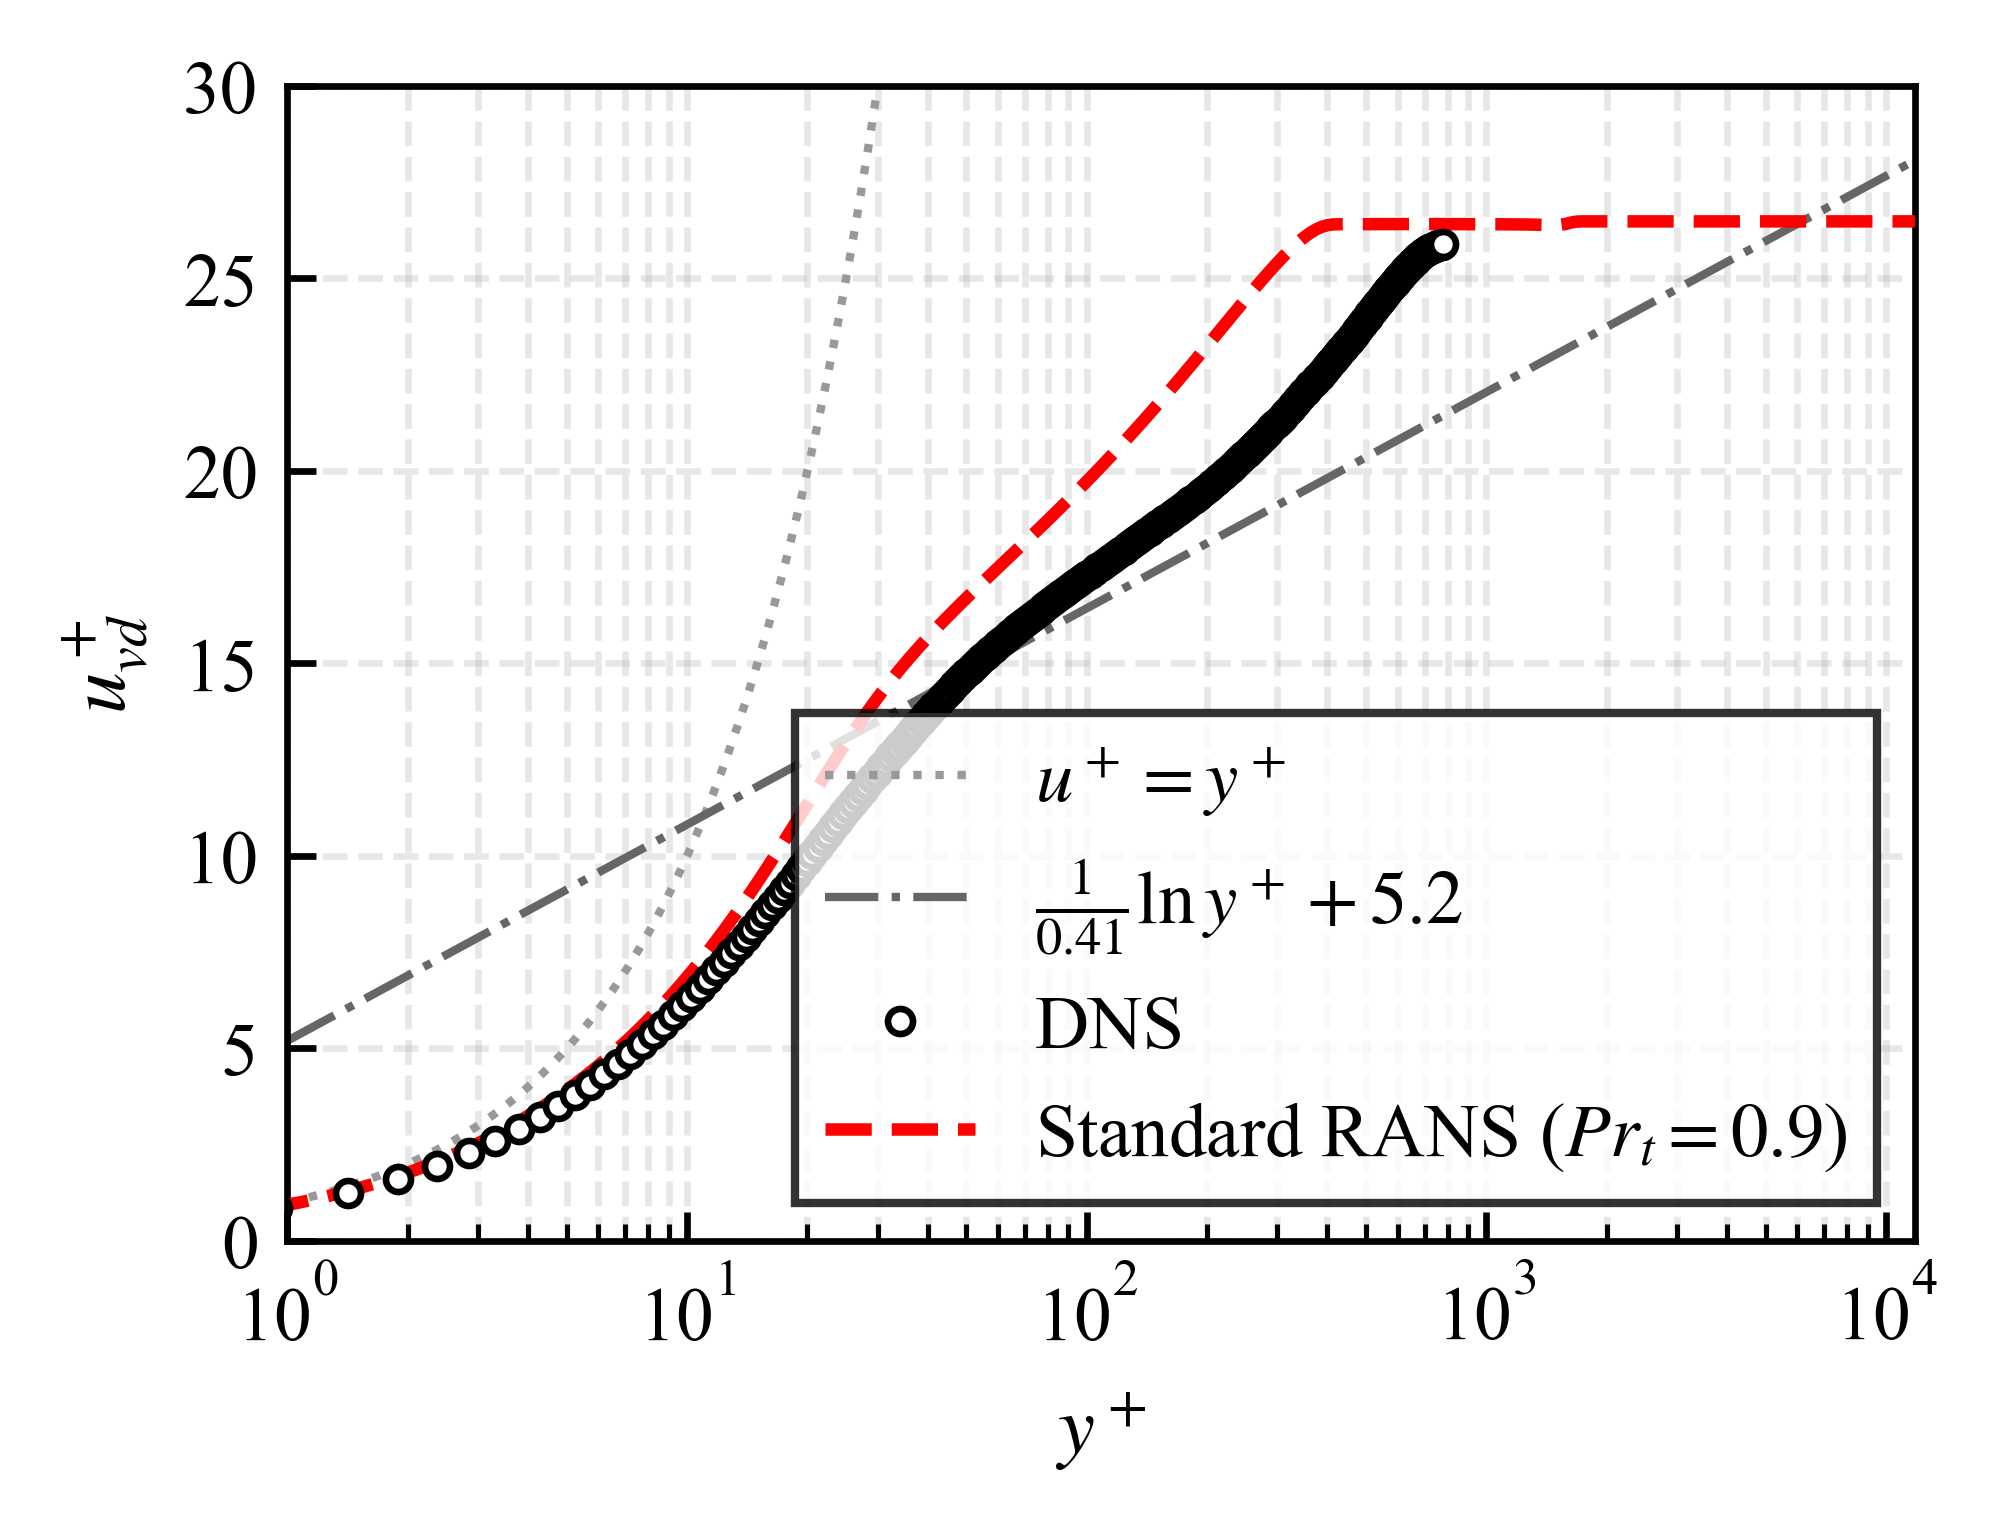
\includegraphics[width=0.62\linewidth]{check1_van_driest_uplus.png}
\caption{Van Driest transformed velocity in wall units. DNS (hollow circles) follows the
log law; the corrected-baseline RANS (red dashed, $\Prt=0.9$) now tracks it, with
$\utau=\SI{63.2}{m/s}$ vs DNS $\SI{67.6}{m/s}$. The calibrated-\Prt{} curve is deferred
to the matched-Re 1B recalibration. The earlier fixed-Re baseline (not shown) sat far
above the log law, which motivated the forensic study in Section~\ref{sec:forensics}.}
\end{figure}

% ---------- Check 2 ----------
\subsection{Check 2 --- \texorpdfstring{$T(u)$}{T(u)} shape vs level (calibration space)}
\textbf{Result: clean pass.} Calibrated RANS collapses onto DNS; the standard
$\Prt=0.9$ error is almost entirely a uniform \emph{level} offset that \Prt{} removes.

\begin{table}[H]
\centering
\begin{tabular}{lccc}
\toprule
 & raw RMSE & level offset & shape RMSE \\
\midrule
Standard ($0.9$)        & 1.279 & $+1.236$ & 0.332 \\
Calibrated ($0.566$)    & 0.293 & $+0.092$ & 0.278 \\
\bottomrule
\end{tabular}
\caption{Shape-vs-level decomposition of the $T(u)$ mismatch
($0.1 < u/U_\infty < 0.9$). The $\Prt=0.9$ error is dominated by the level offset,
confirming \Prt{} as the correct single knob.}
\end{table}

\begin{figure}[H]
\centering
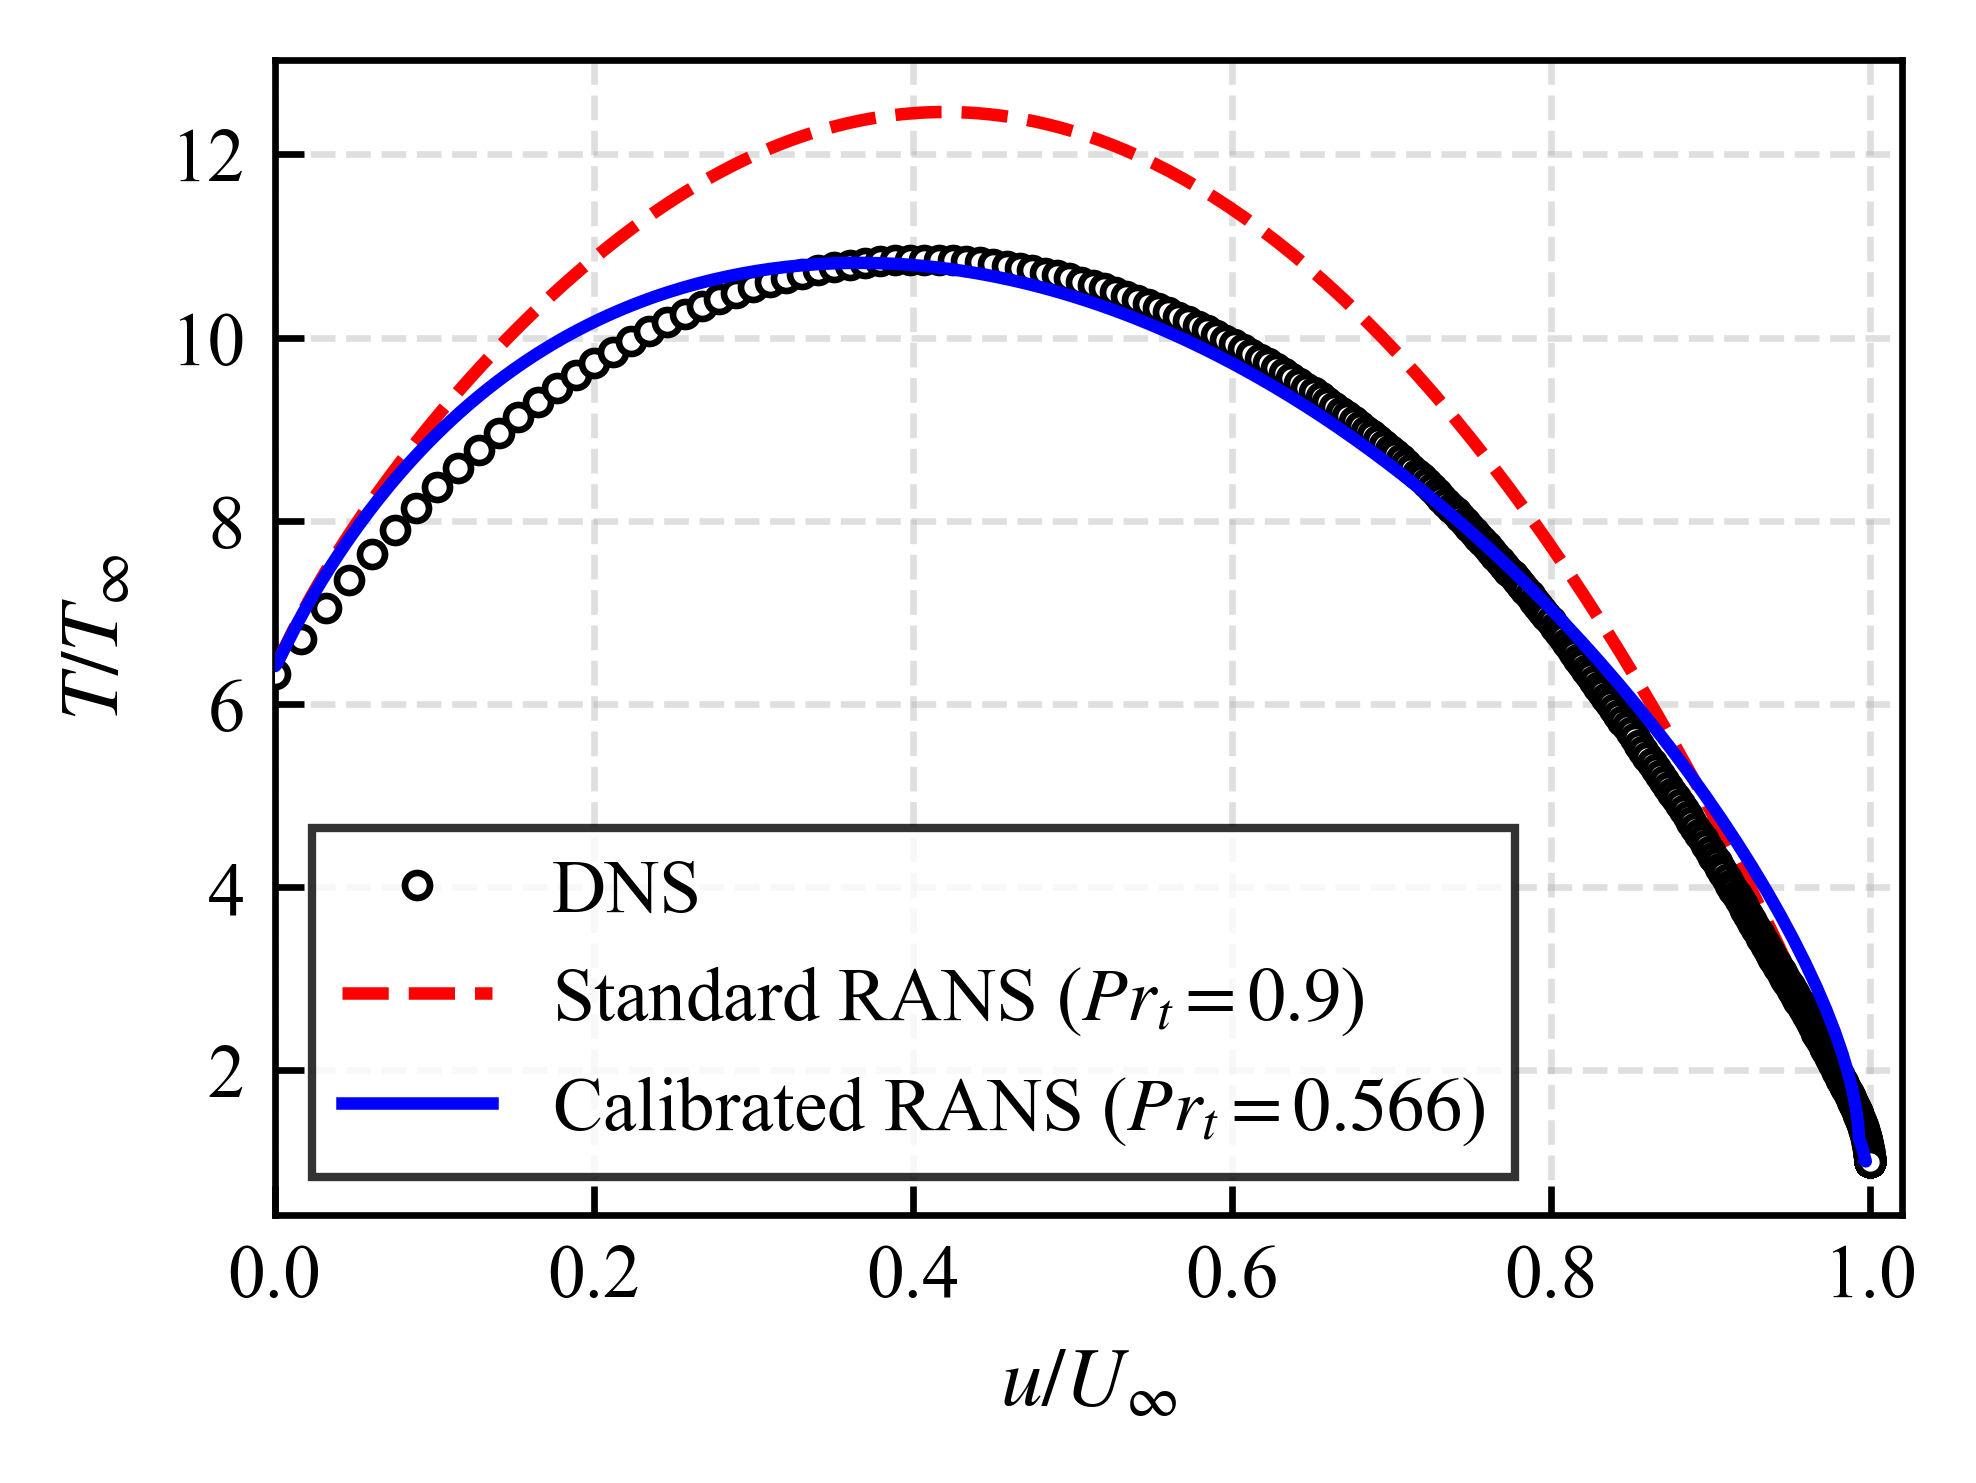
\includegraphics[width=0.62\linewidth]{check2_tu_shape.png}
\caption{$T$--$u$ profiles. Calibrated RANS (blue) overlays DNS (circles); standard RANS
(red) sits too high. Same Crocco--Busemann shape; \Prt{} shifts the level.}
\end{figure}

% ---------- Check 3 ----------
\subsection{Check 3 --- \texorpdfstring{$\Prt$}{Prt}(RANS) vs \texorpdfstring{$\Prt$}{Prt}(DNS) (physical recovery)}
\textbf{Result: supportive, with nuance.} The DNS \Prt{} (column 27) is $\sim 0.8$--$0.95$
in the outer layer but drops to $\sim 0.45$--$0.57$ near the wall. The calibrated
$\Prt = 0.566$ matches the \emph{near-wall} DNS value (which governs wall heat flux) and
lies within $11.5\%$ of the boundary-layer average ($0.639$). Both are far below $0.9$.

\begin{figure}[H]
\centering
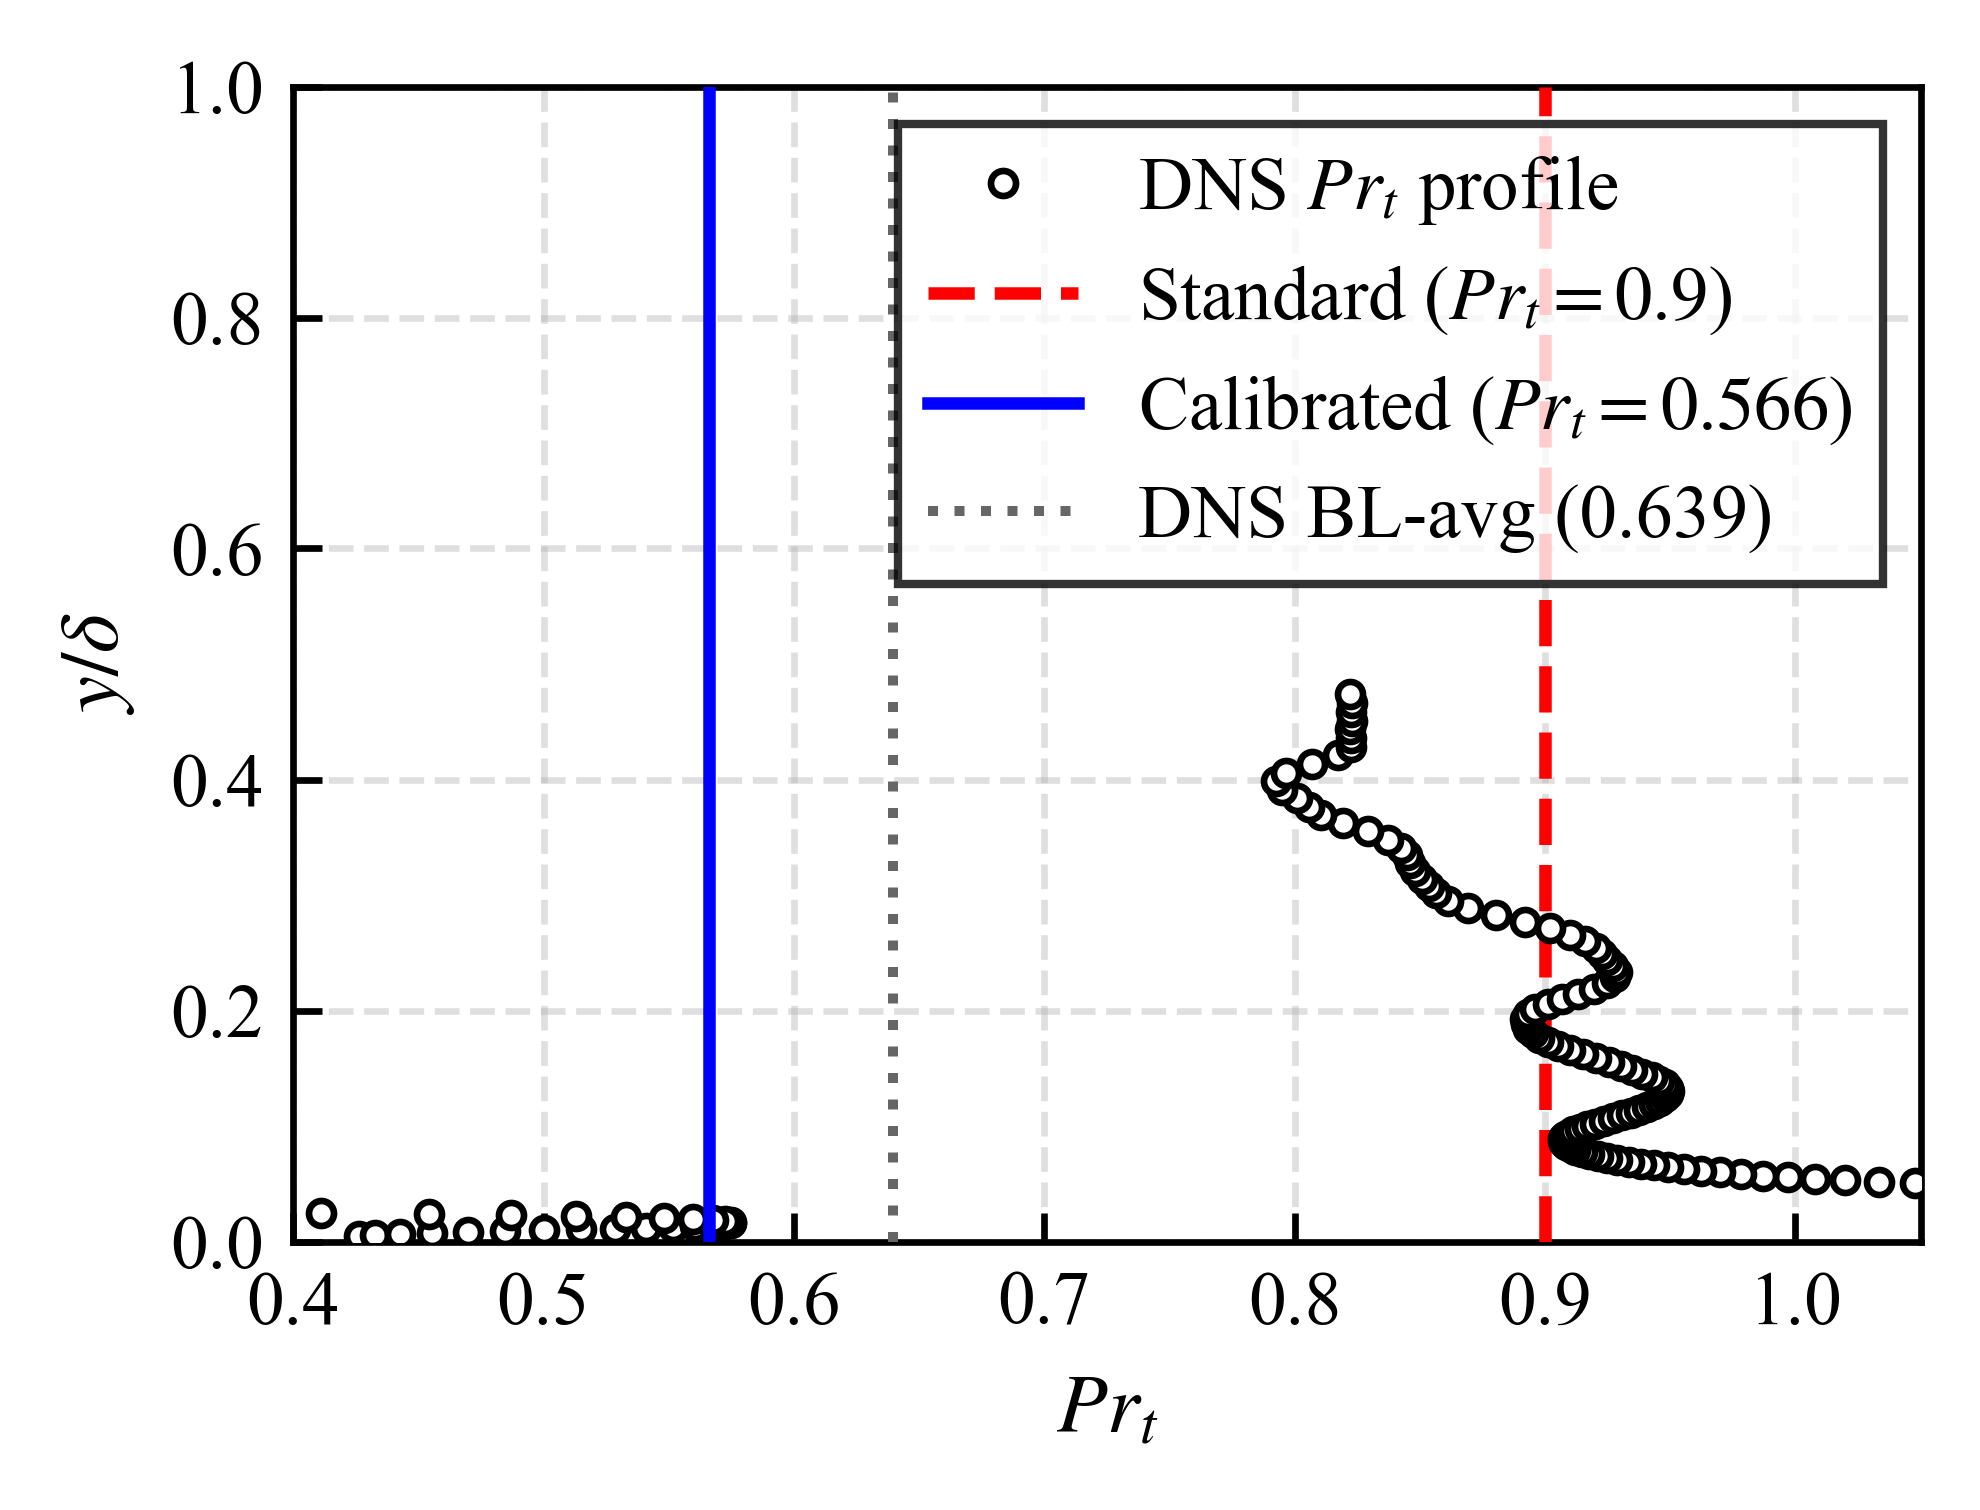
\includegraphics[width=0.62\linewidth]{check3_prt_recovery.png}
\caption{DNS \Prt{} profile with reference lines. The constant calibrated value sits at
the near-wall DNS level; the BL-average is $0.639$.}
\end{figure}

% ============================================================
\section{Wall-Shear Forensics}
\label{sec:forensics}
% ============================================================
The forensic study (\texttt{investigate\_wall\_shear.py}) maps wall and boundary-layer
quantities along the entire plate rather than at a single station. Run on the corrected
derived-Re baseline it confirms a healthy, developing turbulent boundary layer and
explains the small residual gap to the DNS station; on the earlier fixed-Re baseline it
had localized the (now-resolved) wall-shear deficit.

\begin{table}[H]
\centering
\begin{tabular}{lcccc}
\toprule
$x$ [m] & $\delta_{99}$ [mm] & \utau{} [m/s] & $Re_x$ & $Re_\tau$ \\
\midrule
0.25 &  7.4 & 79.1 & \num{2.67e6} & 117.5 \\
0.50 & 12.0 & 71.9 & \num{5.35e6} & 166.9 \\
1.00 & 20.3 & 66.1 & \num{1.07e7} & 252.6 \\
1.50 & 27.8 & 63.2 & \num{1.60e7} & 328.5 \\
1.75 & 31.7 & 62.1 & \num{1.87e7} & 366.2 \\
\bottomrule
\end{tabular}
\caption{Boundary-layer development of the corrected derived-Re baseline ($\Prt=0.9$).
At the analysis station ($x=\SI{1.5}{m}$) $Re_\tau = 328$, versus DNS $Re_\tau = 646$.}
\end{table}

\paragraph{Findings.}
\begin{itemize}[nosep]
  \item \textbf{Momentum field now sound.} With the freestream Reynolds number derived
        from the DNS state (unit-$Re=\SI{1.07e7}{}$/m), the wall shear recovers to
        physical values: $\utau=\SI{63.2}{m/s}$ at $x=\SI{1.5}{m}$ (vs DNS
        $\SI{67.6}{m/s}$), and $C_f(x=\SI{1.5}{m})=\num{4.5e-4}$ sits above laminar
        Blasius ($\num{1.7e-4}$) and below the incompressible-turbulent line
        ($\num{2.1e-3}$)---the expected compressible-turbulent range at Mach 14.
  \item \textbf{Residual Reynolds / flow-state gap (benign).} At $x=\SI{1.5}{m}$,
        $Re_\tau=328$ vs DNS $646$: the RANS boundary layer is still developing
        ($Re_\tau$ grows monotonically from $118$ to $366$ along the plate) and the DNS
        station sits at a higher $Re_\tau$. This is a flow-state difference, not a model
        defect, and is much smaller than in the earlier fixed-Re baseline ($Re_\tau=182$).
  \item \textbf{Near-ZPG, mild viscous interaction.} Wall pressure is \SI{285}{Pa} vs
        freestream \SI{230}{Pa} ($1.24\times$), and $\delta_{99}=\SI{27.8}{mm}$ is
        $\sim 1.4\times$ the incompressible turbulent estimate---close to the clean
        zero-pressure-gradient DNS, far milder than the earlier baseline suggested.
  \item \textbf{No transition / no pathology.} $C_f(x)$ decays monotonically with no
        laminar$\to$turbulent jump; velocity profiles develop smoothly (no separation,
        no relaminarization).
  \item \textbf{Convergence (actionable).} After \num{15000} iterations,
        $\mathrm{rms}[\rho] = -7.1$ but $\mathrm{rms}[\rho E] = -1.63$: the \emph{energy}
        equation---which governs the temperature field we calibrate on---has improved
        over the earlier run ($-0.70$) but is still the limiting field and warrants a
        deeper floor.
\end{itemize}

\begin{figure}[H]
\centering
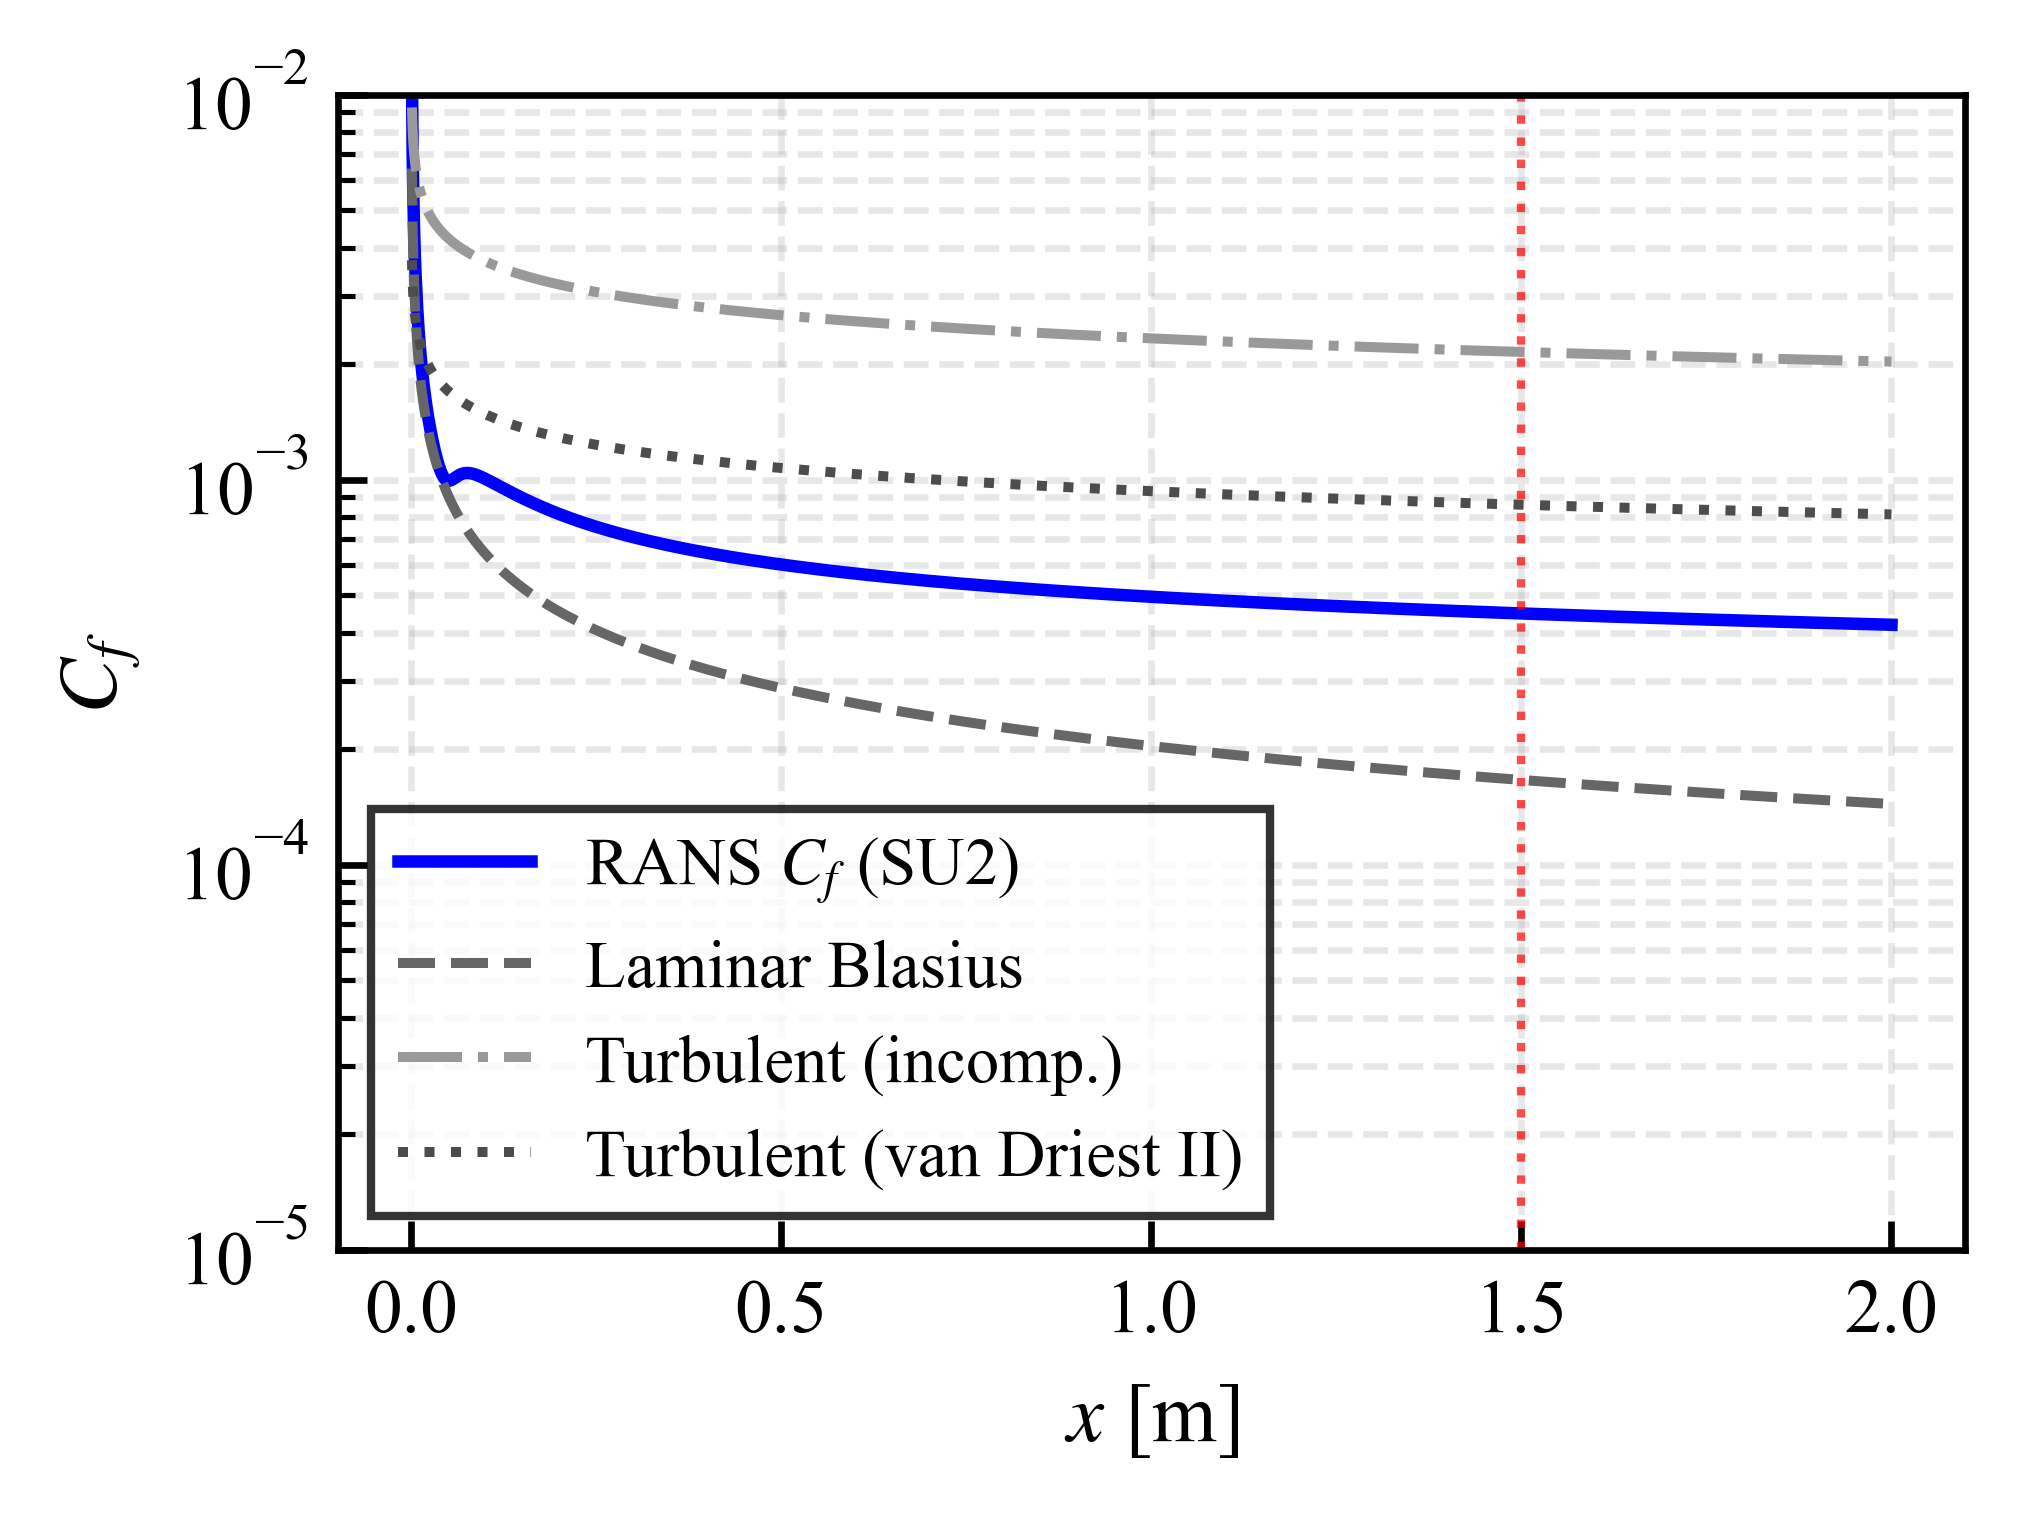
\includegraphics[width=0.48\linewidth]{diag_cf_vs_x.png}\hfill
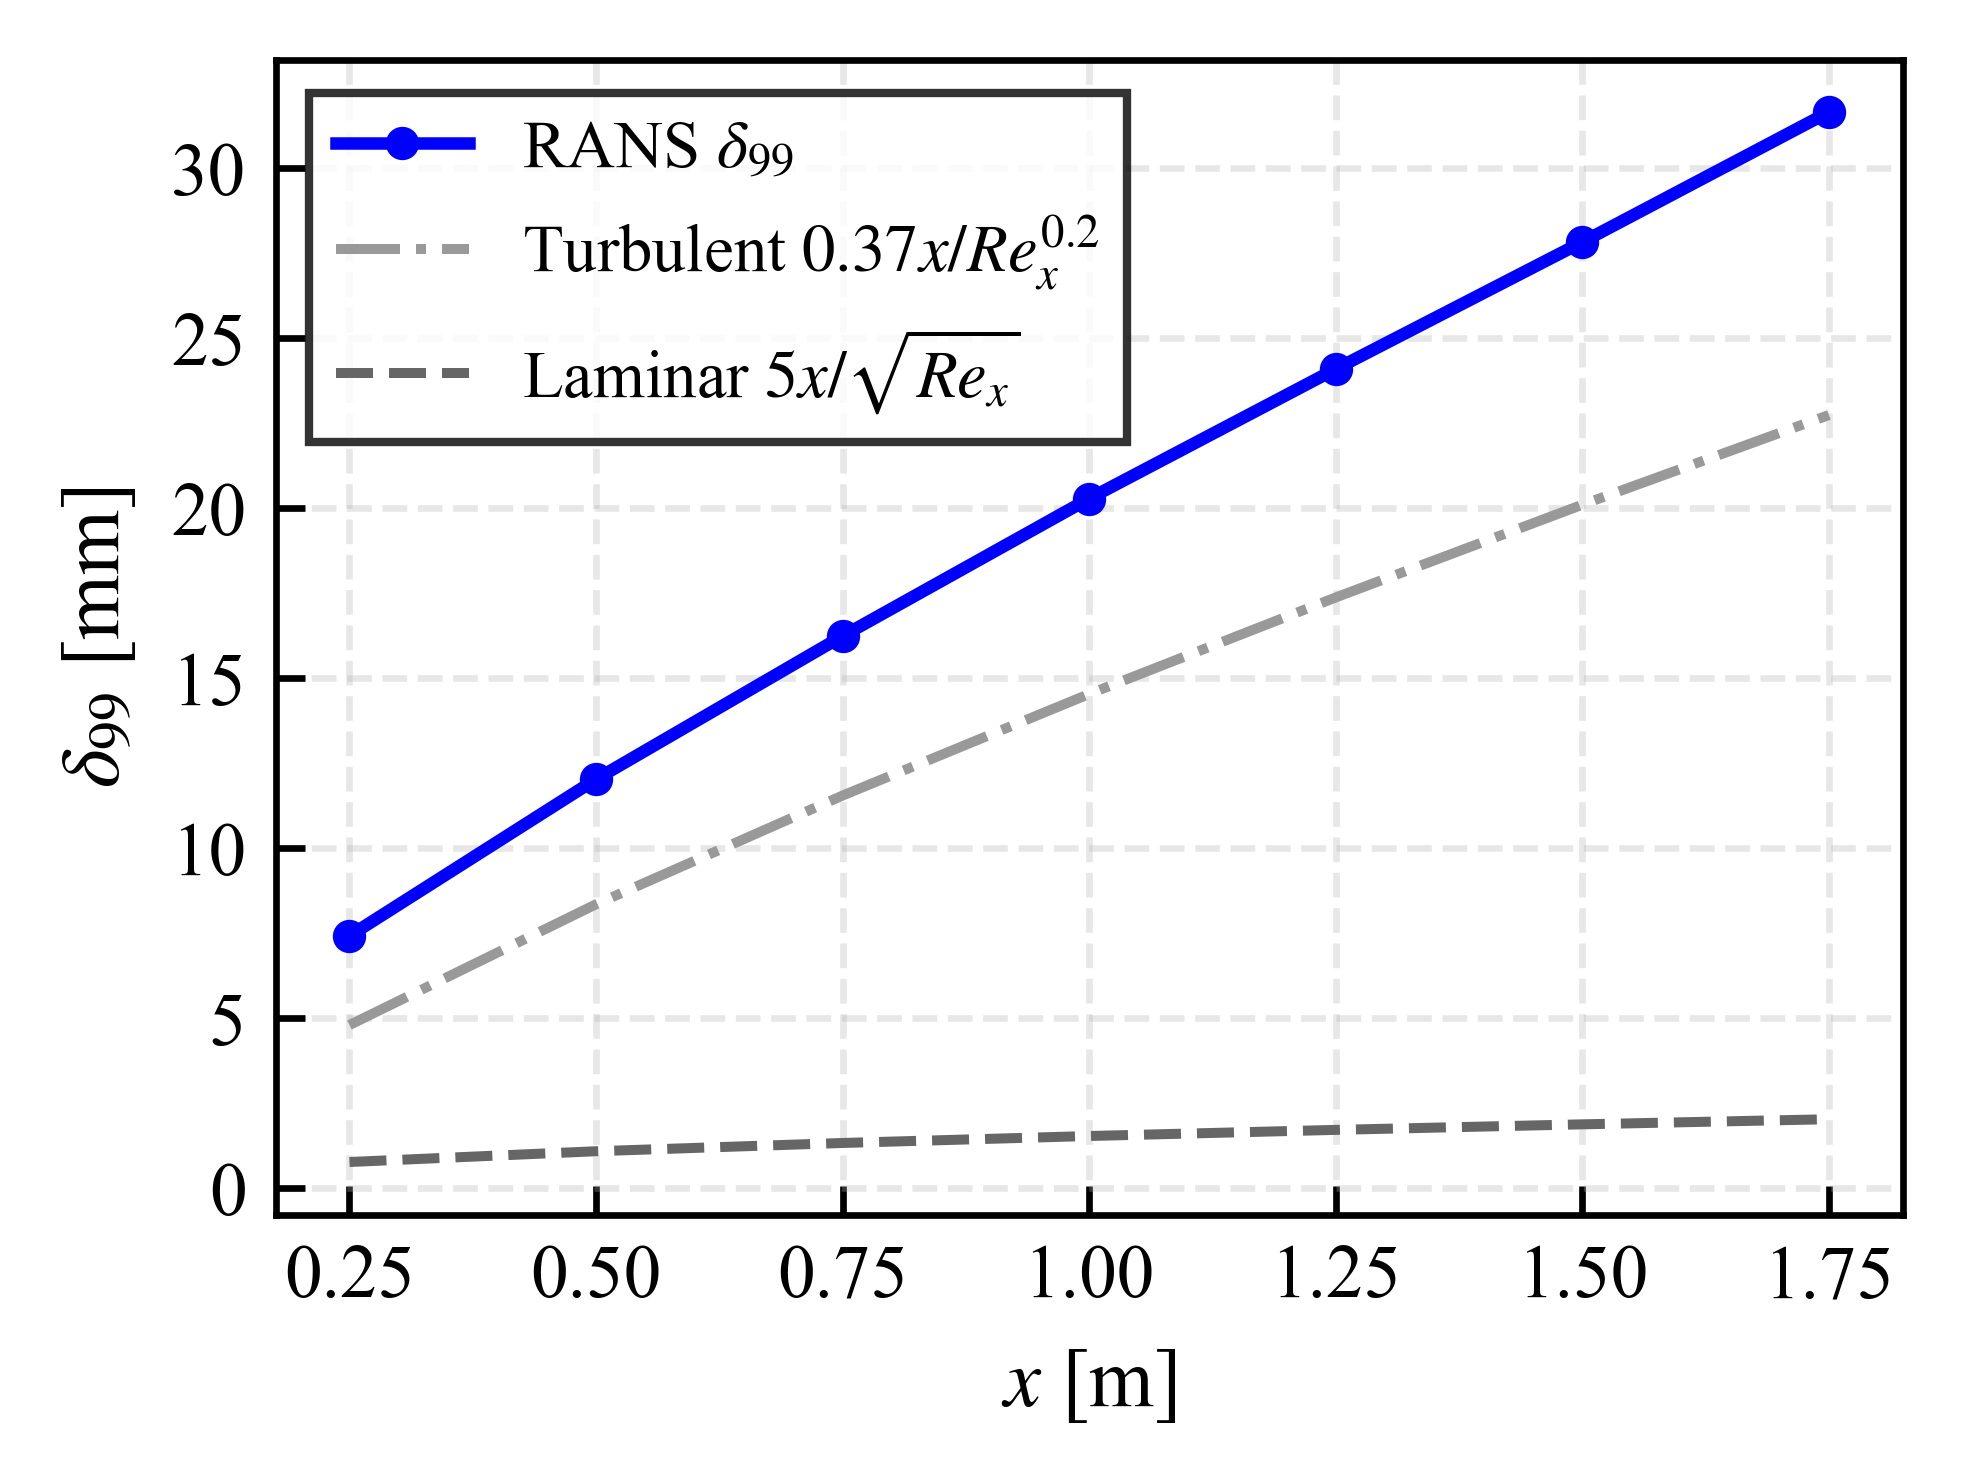
\includegraphics[width=0.48\linewidth]{diag_delta_vs_x.png}
\caption{Left: skin-friction $C_f(x)$ vs incompressible references (monotonic, no
transition; the compressible-turbulent $C_f$ sits between the laminar and
incompressible-turbulent lines). Right: boundary-layer growth $\delta_{99}(x)$, mildly
thicker than incompressible turbulent theory (expected for Mach 14).}
\end{figure}

\begin{figure}[H]
\centering
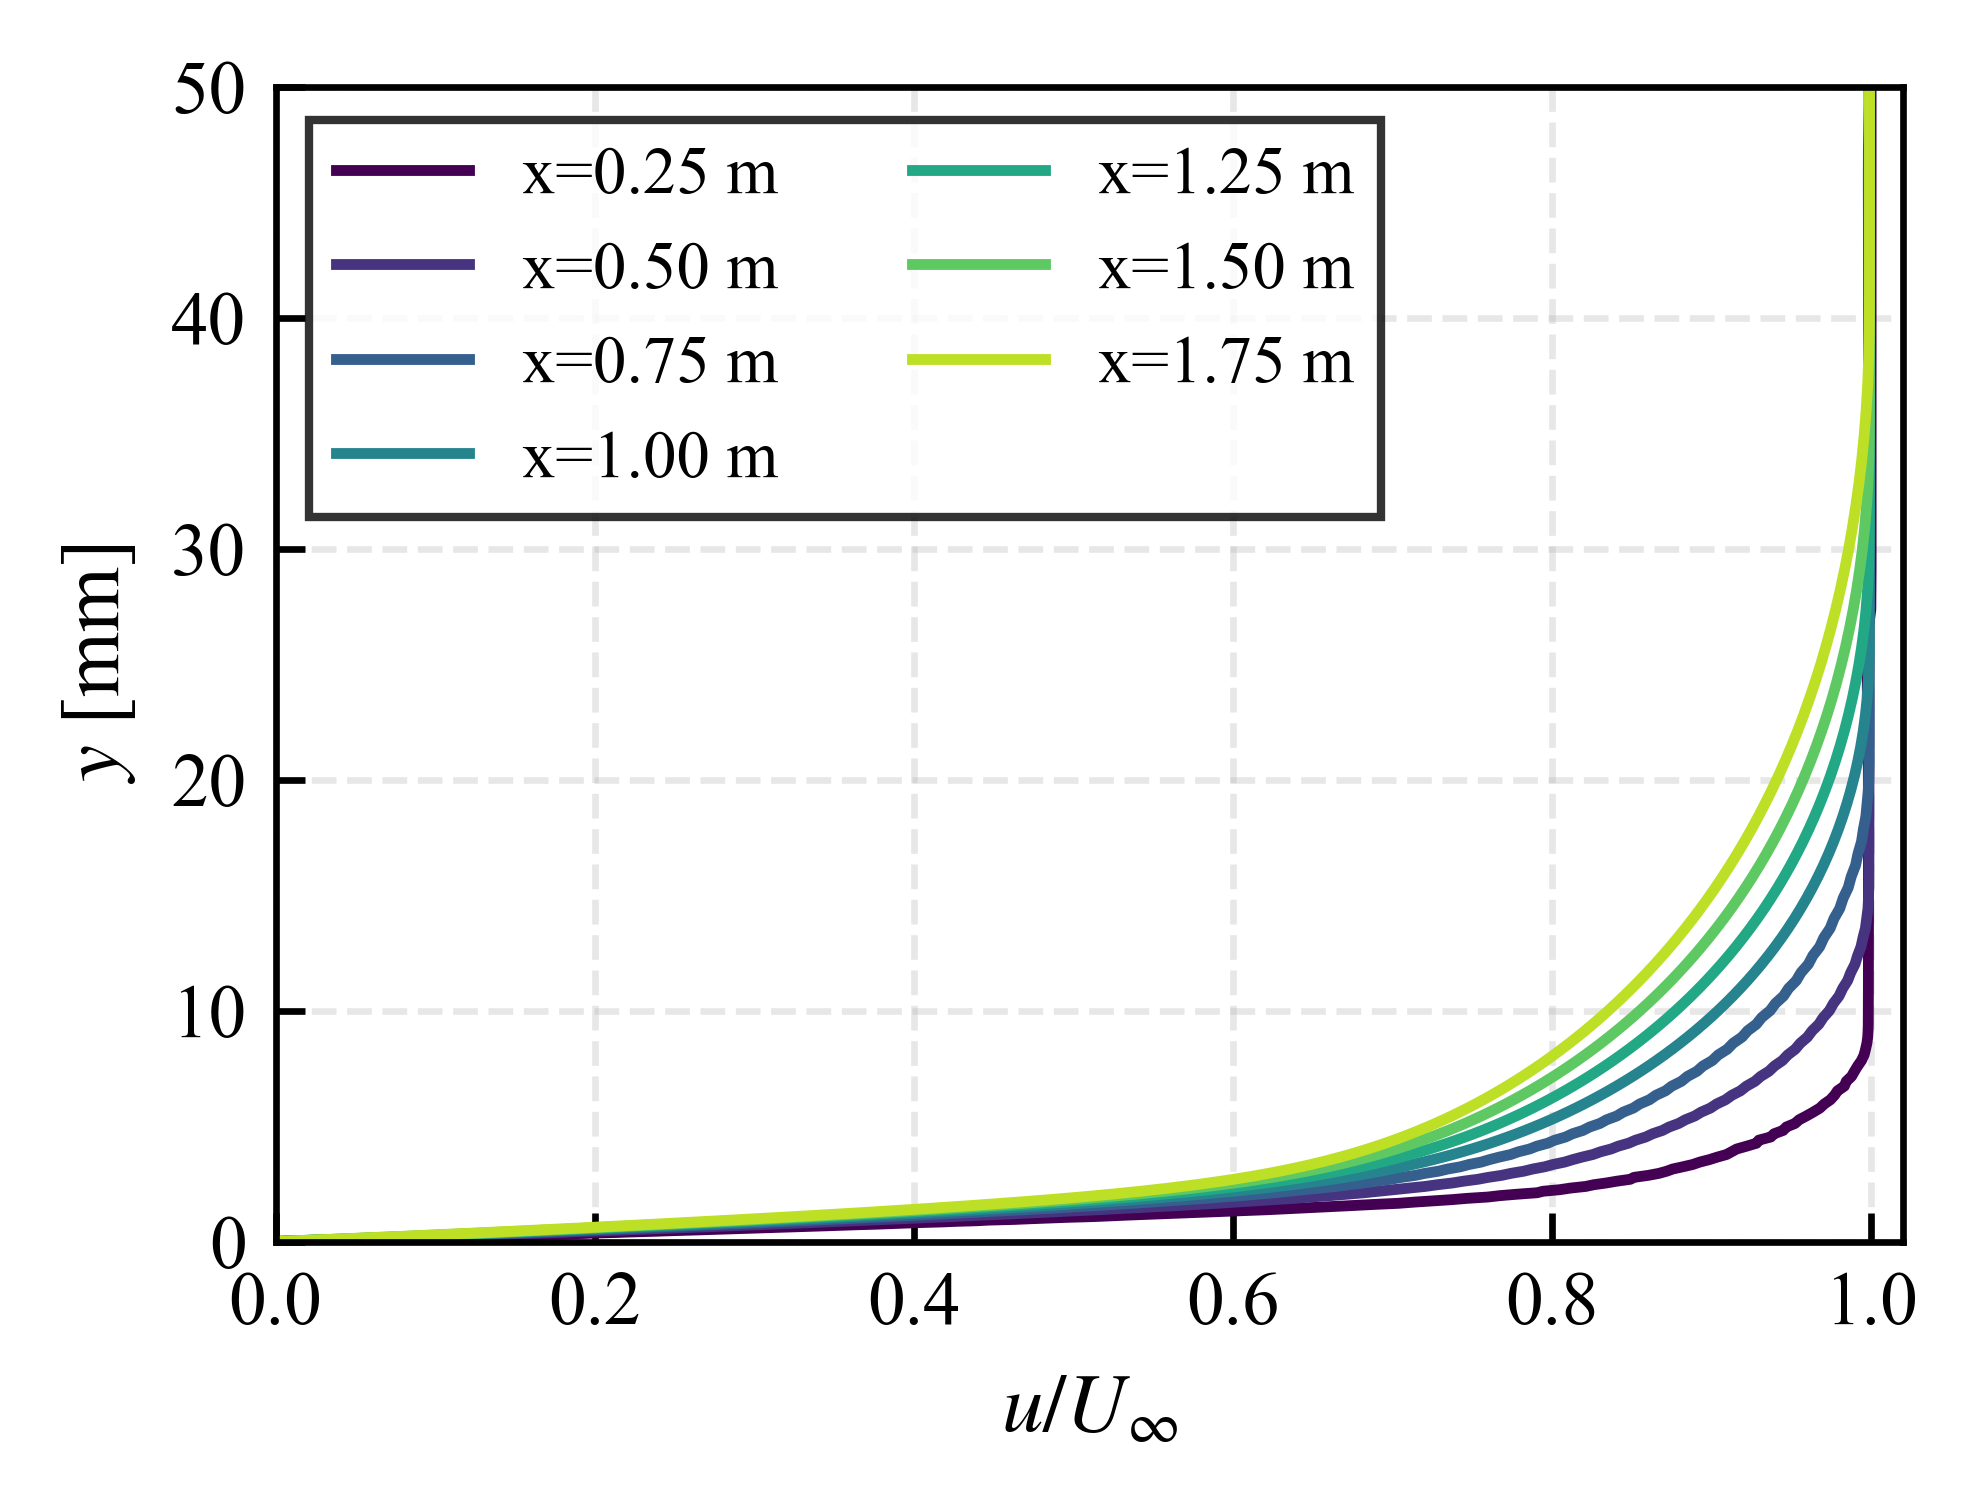
\includegraphics[width=0.55\linewidth]{diag_profiles_vs_x.png}
\caption{Velocity profiles at several stations: smooth, monotonic development; no
numerical pathology.}
\end{figure}

% ============================================================
\section{Verdict}
% ============================================================
With the corrected DNS-consistent baseline the velocity-space concern is
\textbf{largely resolved}: in wall units the RANS momentum field now collapses onto the
DNS/log-law ($\utau = \SI{63.2}{m/s}$ vs DNS $\SI{67.6}{m/s}$), and the wall-shear
forensics show a healthy, developing turbulent boundary layer. The small residual gap to
the DNS ($Re_\tau=328$ vs $646$) is a benign Reynolds-number/flow-state difference---the
RANS plate is still developing---\emph{not} a turbulence-model failure or numerical
pathology. This \emph{reinforces} the methodology twice over: the momentum field
underpinning the calibration is now validated directly, and because the $T(u)$
\emph{shape} is self-similar (only weakly Reynolds-dependent), \Prt{} remains the correct
single knob even where the momentum states differ---though its calibrated \emph{value},
which sets the $T(u)$ \emph{level}, must be fixed at matched Reynolds number (Section~6).
Check 2 (collapse) and Check 3 (physical \Prt{} recovery) therefore rest on a sound
momentum solution, with their numeric values pending the matched-Re recalibration. The
\Prt{} result is a genuine physical correction, not a fudge factor.

% ============================================================
\section{Next Steps and Plan}
% ============================================================
\paragraph{Where this memo stands.} Check~1 and the wall-shear forensics
(Section~\ref{sec:forensics}) use the corrected derived-Re, CFL-250 baseline.
Checks~2--3 and the headline result (Section~1) still use the earlier 1A runs
(fixed $Re=\num{5e6}$). A direct test shows the corrected baseline \emph{already} halves
the $\Prt=0.9$ error in $T(u)$ space (level offset $+1.24\!\to\!+0.58$, raw RMSE
$1.28\!\to\!0.63$ vs DNS) \emph{before any calibration}. Because \Prt{} sets that level,
the calibrated $\Prt=0.566$ and the $-61.3\%$ headline are \textbf{provisional} and
expected to move once recalibrated at matched Reynolds number. Closing this gap is the
immediate next action (item~1).

\begin{enumerate}[nosep]
  \item \textbf{Matched-Re recalibration (1B) --- immediate next step.} Re-run the Brent
        \Prt{} calibration for the M14Tw018 case at the derived Reynolds number and
        CFL~250, refresh \texttt{optimization\_log.csv}, then regenerate Checks~2--3 and
        the Section~1 headline against the corrected baseline and the new calibrated run.
        This replaces the provisional $\Prt=0.566$ / $-61.3\%$ with matched-Re values.
  \item \textbf{Deeper baseline convergence.} The corrected derived-Re baseline reaches
        $\mathrm{rms}[\rho E]=-1.63$ (up from $-0.70$); push further toward
        $\lesssim -5$ and confirm wall-heat-flux (QoI) stationarity.
  \item \textbf{Transform consistency.} Optionally compare against the Trettel--Larsson
        transform (DNS column 26) in addition to van Driest, which is known to collapse
        cold-wall hypersonic profiles better.
  \item \textbf{Resume the core thesis track.} Continue GP + Active Learning multi-point
        calibration across the 5-case DNS family (M2.5--M14), training the surrogate
        $[\,\mathrm{Mach}, T_w/T_{aw}, \theta_{pg}\,] \to \Prt$.
  \item \textbf{Geometry generalization.} Extend to the compression-ramp / SBLI case and
        test whether the calibrated (or GP-predicted) \Prt{} transfers.
\end{enumerate}

% ============================================================
\section*{Appendix: Artifact Inventory}
% ============================================================
\noindent All artifacts live in \texttt{post\_processing/calibration\_diagnostics/}:
\begin{itemize}[nosep]
  \item \texttt{plot\_calibration\_diagnostics.py} --- the three checks.
  \item \texttt{investigate\_wall\_shear.py} --- wall-shear / BL forensics.
  \item Figures: \texttt{check1\_van\_driest\_uplus}, \texttt{check2\_tu\_shape},
        \texttt{check3\_prt\_recovery}, \texttt{diag\_cf\_vs\_x},
        \texttt{diag\_delta\_vs\_x}, \texttt{diag\_profiles\_vs\_x} (PNG + PDF).
  \item This memo: \texttt{calibration\_diagnostics\_summary.tex} $\to$ \texttt{.pdf}.
\end{itemize}

\vspace{0.5em}
\noindent\textbf{Key data.} Optimal $\Prt = 0.566$ (RMSE $0.286$); baseline $\Prt=0.9$
(RMSE $0.739$); DNS BL-avg $\Prt = 0.639$. Corrected derived-Re baseline at
$x=\SI{1.5}{m}$: RANS $\utau = \SI{63.2}{m/s}$ vs DNS $\SI{67.6}{m/s}$;
$Re_\tau = 328$ vs $646$; $\delta_{99}=\SI{27.8}{mm}$; wall $p = \SI{285}{Pa}$ vs
freestream $\SI{230}{Pa}$; unit-$Re=\SI{1.07e7}{}$/m. Convergence:
$\mathrm{rms}[\rho]=-7.1$, $\mathrm{rms}[\rho E]=-1.63$.

\end{document}
